This chapter describes the work still to be done on the project over the coming months.
The project will be advanced in two ways, by generating hardware for it, and modifying the software involved.

\section{Hardware}
\subsection{PCB}
Once the code is functional on the DSP, the next step is to move it off the evaluation board and onto a specially designed PCB.
This will convert the project into a form more resembling a product, and remove any excess hardware as well as adding more required hardware that the evaluation board does not include.
It will also allow for a larger choice in which DSP is used, allowing a faster, more powerful DSP to be selected.

\section{Algorithm}
\subsection{LMS}
\label{sec:LMS}
LMS is a form of adaptive filter.
It works by reducing the average power of the feedback signal by modifying the coefficients in a Finite Impulse Response (FIR) filter.
An example implementation is shown below in figure~\ref{fig:lmsfilter}.
In this implementation the LMS algorithm will be used as the block labelled ``Adaptation algorithm''.
This version also aims for a slightly different effect to the method that will be employed in this project.
This project will be feeding the inverse of the noise estimate, -\^{n}(m), to the listener in order to generate the cancelling in their ear, rather than to remove the noise inside the software.

\begin{figure}[H]
	\centering
	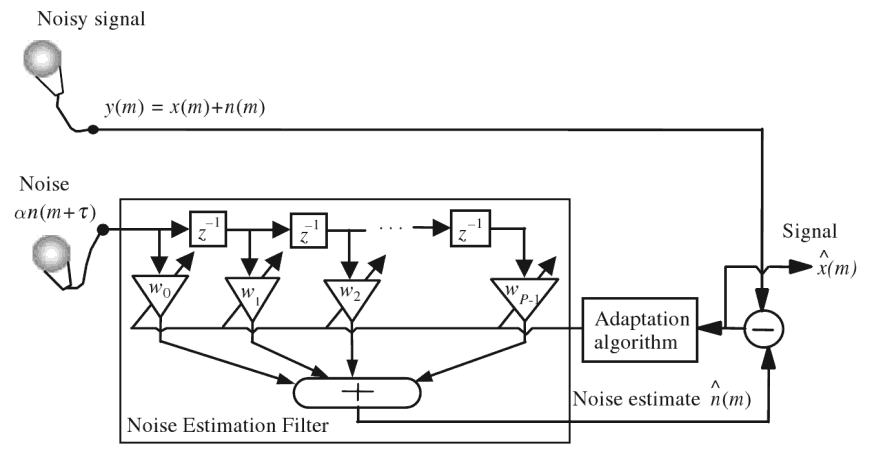
\includegraphics[width=\textwidth]{./img/lmsfilter.png}
	\caption{An example setup for the use of an LMS filter in noise cancellation (Sourced from Advanced Digital Signal Processing and Noise Reduction \cite{AdvancedDSPing})}
	\label{fig:lmsfilter}
\end{figure}

\subsection{ICA}
Independent Component Analysis (ICA) is a method for identifying and separating multiple sound sources without prior knowledge of what they are.
ICA will allow the user to select an undesired input without having to direct a microphone to detect it.
The ICA will separate out the sounds entering the ears and allow the user to select which one is the `nuisance' sound.
This will then be fed into a modified cancellation algorithm to remove it from the mix.
\\
\\
ICA normally requires the use of at least as many inputs as there are signal sources\cite{AdvancedDSPing}.
Hopefully, using information from psychoacoustics, this can be circumvented from the knowledge that the inputs are directional, and accounting for the effect the head has on the signals.
